\newpage
\section{L'algorithme de reconstruction}

\subsection{La méthode}

Pour rappel, l'objectif de l'algorithme est de produire un maillage dense à partir d'un nuage de points LIDAR, fourni au format PLY.

Le fonctionnement de l'algorithme peut se décomposer en quatre phases distinctes :
\begin{enumerate}
 \item Le chargement du nuage de point LIDAR en mémoire
 \item L'échantillonage dans le plan (X,Y) des points
 \item La conversion en matrice d'élévation
 \item La simplification du maillage
\end{enumerate}



\subsection{Acquisition du nuage de points}
Le nuage de points est fourni dans un fichier PLY au format ASCII (il existe une version binaire, plus légère mais plus difficilement lisible), qui contient une série de lignes d'en-têtes, puis le nuage à raison d'un point par ligne, dont les trois coordonnes sont séparées par un espace.

Ne trouvant pas de module existant pour charger ce nuage de point en mémoire (voire directement dans CGAL), j'ai choisi d'écrire mon propre module de lecture de fichier PLY.
Celui-ci renvoie donc pour un chemin vers un fichier PLY, un \texttt{Vector <Point> nuage} ainsi que d'autres informations relatives au nuage (taille, nombre de points).
\begin{figure}[H]
  \centering
   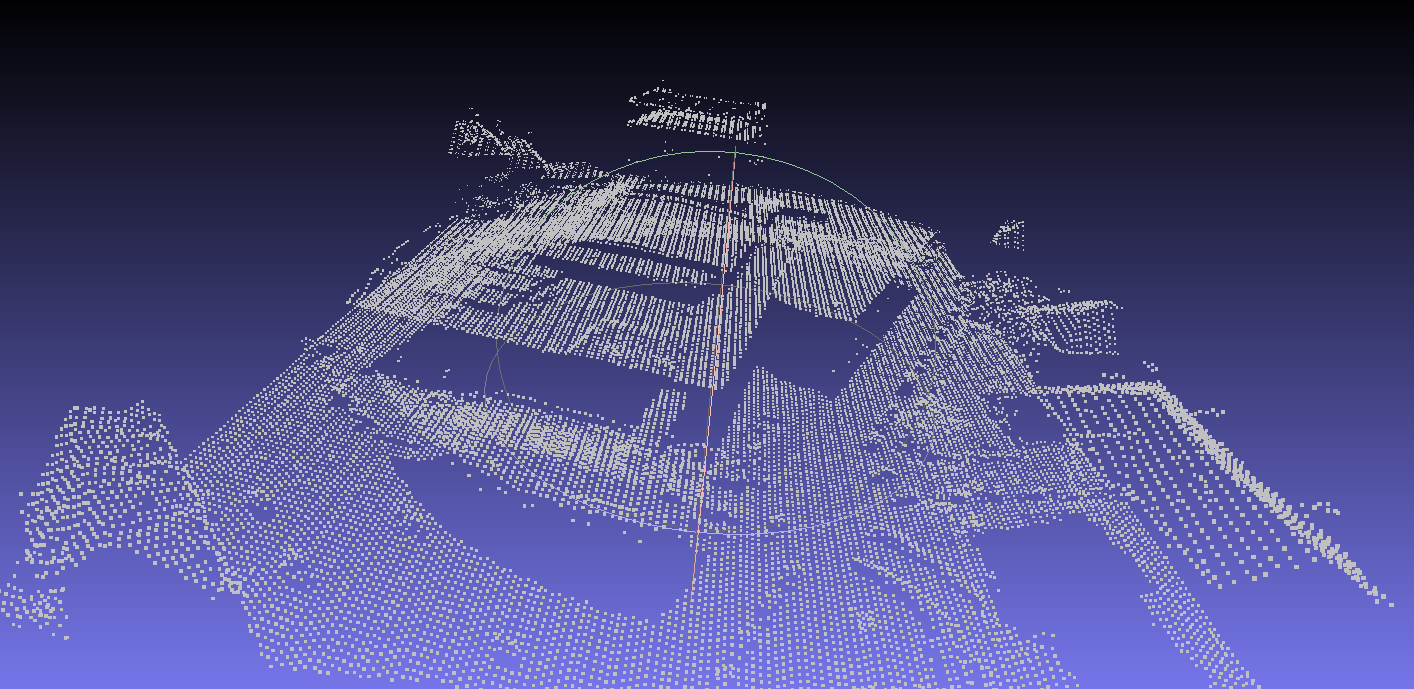
\includegraphics[width=7cm]{nuagePLY.png}
   \caption{Le nuage de points ouvert avec Meshlab}
   \label{nuagePLY}
\end{figure}


\subsection{Échantillonnage}
À partir du nuage de point fourni précédemment, nous allons chercher à calculer la matrice d'élévation, qui en chaque couple de coordonnées (X,Y) associe l'altitude mesurée. Cette matrice serait échantillonnée sur une grille discrète de taille N*N. Les coordonnées seront donc à valeur dans \textlbrackdbl0,N-1\textrbrackdbl.
Le nuage initial étant à coordonnées réelles, il faut dans un premier temps aligner tous les points sur la grille (sur les noeuds de la grille, cf figure \ref{align})
\begin{figure}[H]
  \centering
    \begin{minipage}{.4\linewidth}%
      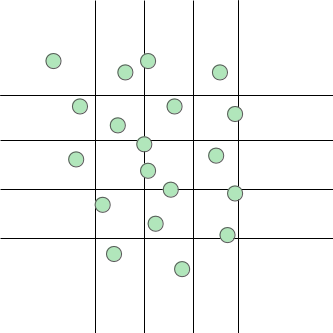
\includegraphics[width=7cm]{align1.png}
    \end{minipage}%
    \begin{minipage}{.2\linewidth}%
    \end{minipage}%
    \begin{minipage}{.4\linewidth}%
      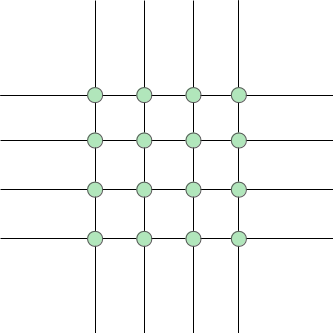
\includegraphics[width=7cm]{align2.png}
    \end{minipage}%
   \label{align}
   \caption{Alignement des points dans le plan (X,Y), sur la grille}
\end{figure}

Chaque point est donc translaté dans le plan (X,Y) vers le noeud le plus proche, tout en conservant sa coordonnée Z.

On se retrouve à la fin de l'échantillonage avec un nuage de point (toujours un \texttt{Vector <Point> nuage} non structuré) mais dont les points sont à coordonnées X et Y discrètes. 

\subsection{Matrice d'élévation}
On va maintenant parcourir chaque point du nuage, et l'ajouter sur une matrice grille, qui est donc de type \texttt{Vector <Point> nuage} : nous obtenons un ensemble structuré qui à chaque noeud de la matrice associe le(s) point(s) associé(s).

Nous parcourons alors cette première matrice grille pour générer la matrice d'élévation (qui à un noeud associe une unique élévation). L'algorithme suivant est utilisé :

\begin{algorithm}[H]
 \KwData{Matrice grille}
 \KwResult{Matrice d'élévation}
 \ForEach{noeud in matrice\_grille}{
  \eIf{nombre de points présents sur ce noeud > 0}{
    matrice\_elevation[noeud]=moyenne\_z(matrice\_grille[noeud])\;
   }{
    \eIf{nombre de points présents sur les 4 noeuds voisins > 0}{
      matrice\_elevation[noeud]=moyenne\_z(matrice\_grille[noeud])\;
    }
    {
      matrice\_elevation[noeud]=altitude\_minimale\;
    }
  }
 }
 \caption{Calcul de la matrice d'élévation à partir de la grille}
\end{algorithm}

\begin{figure}[H]
  \centering
   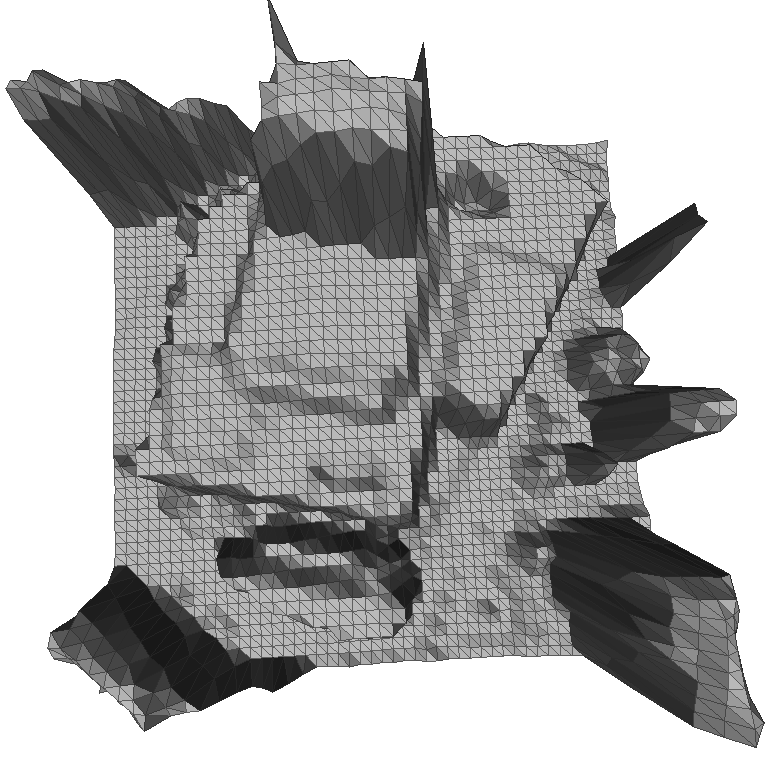
\includegraphics[width=7cm]{matrix.png}
   \caption{La matrice d'élévation}
   \label{matrix}
\end{figure}

Nous obtenons donc une carte d'élévation (discrète), ce qui est cohérent avec la notion de ``vue du ciel'' où tout le plan (X,Y) est visible et associé à une seule coordonnée Z. La figure \ref{matrix} montre un exemple de carte d'élévation.
\subsection{Conversion en Polyhedron\_3D}
Puisque nous allons par la suite utiliser des fonctions de CGAL, il faut convertir cette carte d'élévation en \texttt{Polyhedron\_3D}, qui est une structure CGAL pour décrire des polyèdres tridimensionnels (comme son nom l'indique).

Pour réussir cette conversion, j'ai du utiliser un \emph{incremental builder}, et l'adapter (non sans mal) à mes besoins pour qu'il puisse lire la structure de données de la matrice d'élévation.

Le code est relativement complexe lorsque l'on n'a pas l'habitude d'utiliser CGAL, mais l'explication du code en lui-même est hors-sujet dans ce rapport.

\subsection{Simplification du maillage}
C'est avec la fonction \texttt{edge\_collapse} de CGAL que j'ai pu réduire le nombre de triangles dans le maillage, en préservant la forme générale du maillage.

Pour décrire rapidement le fonctionnement de cette fonction, elle remplace un edge par un vertex, en supprimant et recréant les edges adéquats, et diminuant ainsi le nombre d'arêtes et de triangles.

Cette fonction prend en paramètre un prédicat d'arrêt (qui décidera lorsqu'il faudra arrêter la simplification) et il faut donc décider d'un nombre d'arêtes minimum à conserver.